\chapter{Analysis of the application state}

In this chapter, I will introduce an educational web application helping teach database systems subject at the university.
Furthermore, I will describe the current and planned state of the application from the perspective of software architectural patterns and the used core set of technologies with a focus on the frontend. The goal is to identify the existing problems of the current application, outline how they will be solved in a new portal, as well as indicate what difficulties we can face developing the new application using a new stack of technologies and new architecture.

%%%%%%%%%%%%%%%%%%%%%%%%%%%%%%%%%%%%%%%%%%%%%%%%%%%%%%%%%%%%%%%%

\section{The BI-DBS portal}
The BI-DBS portal is a web application used for teaching database systems subject in a bachelor's study program at the Czech Technical University at the Faculty of Information Technology. The portal is complex and has many useful functionalities. It allows managing and tracking all the student's studying progress during the semester, including semester tests, complex semester work, and exams. Besides, teachers have an overview of all their student's work in one application.\\
The current application was developed, as well as a new one being developed by students and teachers in subjects BI-SP1, BI-SP2 subjects, and bachelor and master theses. That is a unique fact about this project. Every year, new students begin working on application development. They are open to sharing their ideas for improving the application. Thus, we are designing and implementing a better and better product each year.

%%%%%%%%%%%%%%%%%%%%%%%%%%%%%%%%%%%%%%%%%%%%%%%%%%%%%%%%%%%%%%%%

%%%%%%%%%%%%%%%%%%%%%%%%%%%%%%%%%%%%%%%%%%%%%%%%%%%%%%%%%%%%%%%%

\section{Current state of the application}
The current BI-DBS portal was deployed for the first time in 2016. Over time it gained new features and grew large. Used technologies became less relevant and it became difficult to maintain it.

\subsection{Architecture}
The current application was built in a traditional way, using a monolithic architecture approach and following the Model-View-Presenter architectural pattern\cite{potel_mvp}. Figure 1.1 shows the visualization of the architecture. The application is presented as one monolithic unit, and it is composed  of three components. 

\begin{itemize}
  \item The model: Communicates with the database and handles domain and business logic.
  \item The view: Provides visualization and directs user commands to the presenter, does not contain logic.
  \item The presenter: Manages interactions between the database and the view. Receives data from the model and formats it to display in the view.
\end{itemize}

\begin{figure}[hp]
\centering
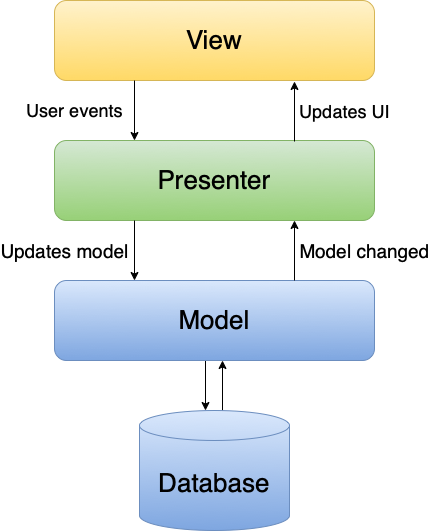
\includegraphics[scale=0.52]{../png/mvp_monolithic.png}
\caption{Monolithic architecture, MVP pattern}\label{picture:mvp}
\end{figure}

\noindent This architecture's main concept is having one code base that benefits in \\ simplifying development, testing, debugging, and deployment. \\
However, we can have those benefits only until the application grows large. Then all those processes get slower, more complex, and become problematic. In addition, with a lack of flexibility and scalability, it becomes challenging to maintain the application and keep it secure. \\

\noindent The BI-DBS portal is being developed by students. Students generally do not have much experience developing large applications and dealing with complex dependencies. Besides, they have limited time to progress in learning and developing the portal. Therefore it takes a lot of time for students to learn before contributing to the project. Thus it is more challenging to keep the application maintainable and ... (just one more example)


%%%%%%%%%%%%%%%%%%%%%%%%%%%%%%%%%%%%%%%%%%%%%%%%%%%%%%%%%%%%%%%%


\subsection{Technologies}
\paragraph*{PHP.} PHP is a general-purpose, open-source scripting language that can be integrated into HTML. It differs from client-side scripting languages in that its HTML is generated on a server and then sent to a client. That feature allows rapidly building a web application with a thick server and thin client. This is one of the approaches to using PHP to build an application, and it is used in the current project. \\
Using his approach leads to creating dependencies between the user interface and the application logic, that make any changes more effortful since a developer needs to adjust it on the both sides.

\paragraph*{Doctrine.} "Doctrine ORM is an object-relational mapper for PHP 7.1+ that provides transparent persistence for PHP objects. It sits on top of a powerful database abstraction layer. One of its key features is the option to write database queries in a proprietary object-oriented SQL dialect called Doctrine Query Language."\\ 
This framework did not cause any problems during the development process and does not have any valuable disadvantages for the BI-DBS to operate properly.

\paragraph*{Nette.} Nette is an open-source framework for creating web applications in PHP. It helps with developing both the client and server sides of the application and also reduces security vulnerabilities.\\ 
Frontend and backend dependencies are strengthened, indicating that they are a single unit. The fact that the they are so strongly dependent is a drawback. Because of this, it is difficult to make changes to one side without having an impact on the other.

\paragraph*{Latte.} Nette framework uses a template system Latte. It compiles templates down to the optimal PHP code.

\paragraph*{AdminLTE.} AdminLTE is a fully responsive administration template. Based on Bootstrap 4.6 framework and also the JS/jQuery plugin. 

\paragraph*{Vue 2.} Vue.js is a javascript framework for building user interfaces and single-page applications.\\
Most of the frontend is implemented using Latte templates and AdminLTE bootstrap. However, in order to reduce dependencies between the frontend and the backend, and also modernize it, few components were refactored to the Vue.js version 2. The logic is defined using the Options API. It is traditional object-oriented way, and up until Vue 2 it was the only way to create components in Vue.

\paragraph*{Javascript.} JavaScript is high-level programming language used for defining the behavior of webpages. It is a dynamically-typed scripting language that enables you to control multimedia, animate graphics, and generate dynamically changing content.\\ 
In the current BI-DBS portal it is used for defining logic on the frontend. Dynamically-typed languages are easy for development, but this feature reduces the code's readability, require more testing and are prone to run-time errors. Large applications like BI-DBS are likely to experience problems as a result of its drawbacks because it is better suited for smaller applications with simple logic.

%%%%%%%%%%%%%%%%%%%%%%%%%%%%%%%%%%%%%%%%%%%%%%%%%%%%%%%%%%%%%%%%

%%%%%%%%%%%%%%%%%%%%%%%%%%%%%%%%%%%%%%%%%%%%%%%%%%%%%%%%%%%%%%%%

\section{Planned state of the application} The main reason of creating a new application instead of refactoring the current one is a change of the application's architecture. A new modernized architectural design of the BI-DBS portal was composed by Ing. Andrii Plyskach in his master thesis\cite{mt-plyskach}. We are aiming to correct all the mistakes made in the current application. It is essential to ascertain that we have chosen the right stack of technologies according to the newly chosen architecture.

\subsection{Architecture}
Microservices architectural pattern\cite{architecture-haris} is based on the concept of a series of loosely-coupled services. They can be developed using different technologies and deployed independently. It is more complex architecture than a standard monolithic one. You can see the diagram illustrating microservices architecture in figure 1.2. 

\begin{figure}[hp]
\centering
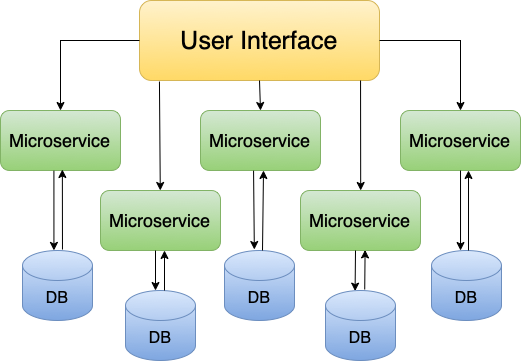
\includegraphics[scale=0.67]{../png/microservices.png}
\caption{Microservice architecture}\label{picture:mvp}
\end{figure}


\paragraph*{Advantages:}
\begin{itemize}
  \item \emph{Code readability:} When services are not strongly dependent the code appears to be better structured and easier for understanding and that is the crustal benefit for the BI-DBS portal.
  
  \item \emph{Independency in choosing a stack of technologies:} Microservices can be developed using different technologies which can be chosen according to the each microservice functionallity without affecting other microservices.
  
  \item \emph{Faster deployments:} Since all microservices can be deployed independently the deploying part is much smaller and the time for deploying one service is rather shorter.

  \item \emph{Fault tolerance:} Because of loose-coupling failing one of the microservices will not bring down the entire application.
\end{itemize}

\paragraph*{Disadvantages:}
\begin{itemize}
  \item \emph{Difficult debugging and testing:} Each service needs to be first tested separately and only then as one unit. Besides it is more difficult to track down errors.

  \item \emph{DevOps required:} To benefit from the fast deployment it should be configured and maintained. It requires the knowledge of development operations.

  \item \emph{Longer development time and limited reuse of code:} Microservices need to be managed separately, therefore it requires more time.
\end{itemize}

%%%%%%%%%%%%%%%%%%%%%%%%%%%%%%%%%%%%%%%%%%%%%%%%%%%%%%%%%%%%%%%%%%%%%%%


\subsection{Technologies}

\paragraph*{PHP.} Since version 5.0, PHP supports object-oriented functionality\cite{php-oop}. PHP is easy to learn, flexible, and supports all required functionalities for our application. It is used in a new project for a domain and business logic on the backend for API implementation.

\paragraph*{Symfony.} Symfony is a powerful back-end framework for creating complex applications which consists of reusable components.\cite{symphony-doc} Thanks to Doctrine Symfony provides all of the tools required to use databases in the application. It is constantly growing and improving, besides it has a strong community. It is easy to learn and has well-written documentation.


\paragraph*{Vue 3.} When the decision to create a new BI-DBS portal has not yet been made its frontend was getting modernized by rewriting components to Vue.js version 2. In the new project, it was chosen to carry on using the Vue.js framework but use a new version 3. This version comes with certain advantages for the application.\cite{vue3-updates}

\paragraph*{New features:}
\begin{itemize}
  \item \emph{Composition API:} Composition API is a set of APIs that allow us to create Vue components by importing functions rather than defining options. Mainly it benefits our project better code organization thus makes a project better structured and code easier to read. Moreover, Composition API enables efficient logic reuse.\cite{compositionapi-doc}
  
   \item \emph{Vite:} Vite is fontend build tool from the cratetor of Vue.js - Evan You. It is module bundler which is built on top of webpack, it will bundle the entire project on startup, hot reloads, and compilation. The primary purpose for the change is for speed. The server starts instantly since it uses native browser support for JavaScript modules.\cite{vite-doc}

   \item \emph{Increased rendering performance.}

\end{itemize}

\paragraph*{Typescript} Typescript is based on JavaScript which is dynamically typed. TypeScript has an additional syntax that makes it statically typed. That has advantages in catching errors during development. It also gives a code more structure and makes it predictable. Typescript is more suitable for big applications than JavaScript. For our project, it is crucial to write code that will be easy to read.\cite{typescript-doc}

\paragraph*{Quasar} Quasar is a web framework based on Vue.js. It provides us with ready-to-use components which are customizable and easy-extendable. Moreover, it makes the application less vulnerable to XSS attacks due to its escaping feature. When using Quasar, developers do not need deep knowledge of CSS and scripting languages to build a good-looking  and responsive application. Besides, it is suitable for developing single-page applications(SPA).\cite{quasar-doc}

\paragraph*{Pinia} Pinia is a Vue.js storage library and state management framework. It is mainly designed for the development of front-end web applications, and it uses declarative syntax as well as its own state management API.\cite{pinia-wiki}

%%%%%%%%%%%%%%%%%%%%%%%%%%%%%%%%%%%%%%%%%%%%%%%%%%%%%%%%%%%%%%%%

%%%%%%%%%%%%%%%%%%%%%%%%%%%%%%%%%%%%%%%%%%%%%%%%%%%%%%%%%%%%%%%%